% !Mode:: "TeX:UTF-8"
% !TEX program  = xelatex


\documentclass{cumcmthesis}
\usepackage[framemethod=TikZ]{mdframed}
\usepackage{url}   % 网页链接
\usepackage{subcaption} % 子标题
\usepackage{float}
\usepackage{enumitem}

\begin{document}

\tableofcontents

% \newpage

\section{引言}

我们可以将上述管道铺设问题用一个连通无向图$G=(V,E)$来表示,这里的$V$是针脚的集合,$E$是针脚之间的可能连接,并且对于每条边$(u,v)\in E$,我们为其赋予权重$w(u,v)$作为连接针脚$u$和针脚$v$的代价,我们希望找到一个无环子集$T\subset E$,既能够将所有节点连接起来,又具有最小的权重,即
$$w(T)=\sum\limits_{(u,v)\in T}{w(u,v)}$$
的值最小。由于$T$是无环的,而且连通所有的节点,因此,$T$必然是一个树形物。我们称这样的树为生成树,为求管道铺设的最短里程,即要求铺设管道的最小生成树。在本题中,我们用两供水站之间的距离表示线的权重:
$$L(u,v)=\sqrt{(x_{u}-x_{v})^{2}+(y_{u}-y_{v})^{2}}$$

贪心策略:
集合$A$是某最小生成树的一个子集,总是保持无环状态。若将边$(u,v)$加入到集合$A$中,使得$A$不违反循环不变式,即$A\cup{(u,v)}$也是某棵最小生成树的子集,则称该边为安全边。该策略应符合一下规则:
\begin{itemize}
  \item 算法执行的任何时刻,图$G_{A}=(V,A)$是一个森林,$G_{A}$中的每个连通分量是一棵树,算法开始时,集合$A$为空集,森林中包含$|V|$棵树,每棵树只有一个节点。
  \item 对于集合$A$为安全的边所连接的是$G_{A}$中不同的连通分量,因此每执行一次循环,减少一棵树。
  \item 循环共执行$|V|-1$次,当整个森林仅包含一棵树时,终止循环。
\end{itemize}

\subsubsection{Prim算法}
  Prim算法是从单个起始点构成的树结构开始,向树结构逐条添加边线以生成树。也就是说,Prim最小生成树是从一个具有n个顶点的带权无向完全图中选择n-1条边并使这个图连通,同时使生成树的权值最小。Prim算法从图中的一个顶点开始,把这个顶点包含在一个集合中,反复寻找一个顶点已在该集合中而另一个顶点还不在该集合中的最小权边,把新边和新节点归并到生成树中,找到这个连通图的最小生成树。在连接节点边数较多时,使用Prim算法较为合适。

  集合A是一棵树,每次加入到A中的安全边永远是连接A和A之外某个节点的边中权重最小的边,采用广度优先搜索的思想——当从Q中取出一个点u时,即要检查u的所有相邻的点,并更新相关的点,Prim算法与分支限界法类似,利用广度优先搜索和优先队列思想,只不过是没有使用分支限界思想。因为可以证明贪心选择性质,使之可以组成一个最优解。
  
\begin{itemize}
  \item 输入:一个加权连通图,其中顶点集合为$V$,边集合为$E$;

  \item 初始化:$Selected = \{x\}$,其中x为集合V中的任一节点(起始点),$Edges = \{\}$,为空;
  
  \item 重复下列操作,直到$Selected = V$:
  \begin{itemize}
    \item 选取权值最小的边$<u, v>$,其中$u \in Selected$,而$v \in V-Selected$;
  
    \item 将$v$加入集合$Selected$中,将$<u, v>$边加入集合$Edges$中;
  \end{itemize}
  \item 输出:使用边集$Edges$来描述所得到的最小生成树。
\end{itemize}

\subsubsection{分级Prim算法}
由于一级水站只能又中心供水站或者其他一级供水站供水,所以我们采用分两级的Prim算法:
\begin{itemize}
  \item 1级Prim算法:输入$V = \{A\}\bigcup \{ V[i]|i=1,2,...N_1\}$,初始化$Selected = \{A\}$。
  输出:边集$Edges1$

  \item 2级Prim算法:输入$V = \{V[i]|i=1,2,...N_1\} \bigcup \{A[i]|i=1,2,...N_2\}$,初始化$Selected = {A}$。输出:边集$Edges2$
  \item 使用边集$Edges1, Edges2$来描述所得到的整个最小生成树。
\end{itemize}
\subsection{问题1模型的求解}
  根据题目要求,我们求出了使得各级管道铺设距离最小的建设方案,如\cref{fig:solution1}所示:
  \begin{figure}[!h]
    \centering
    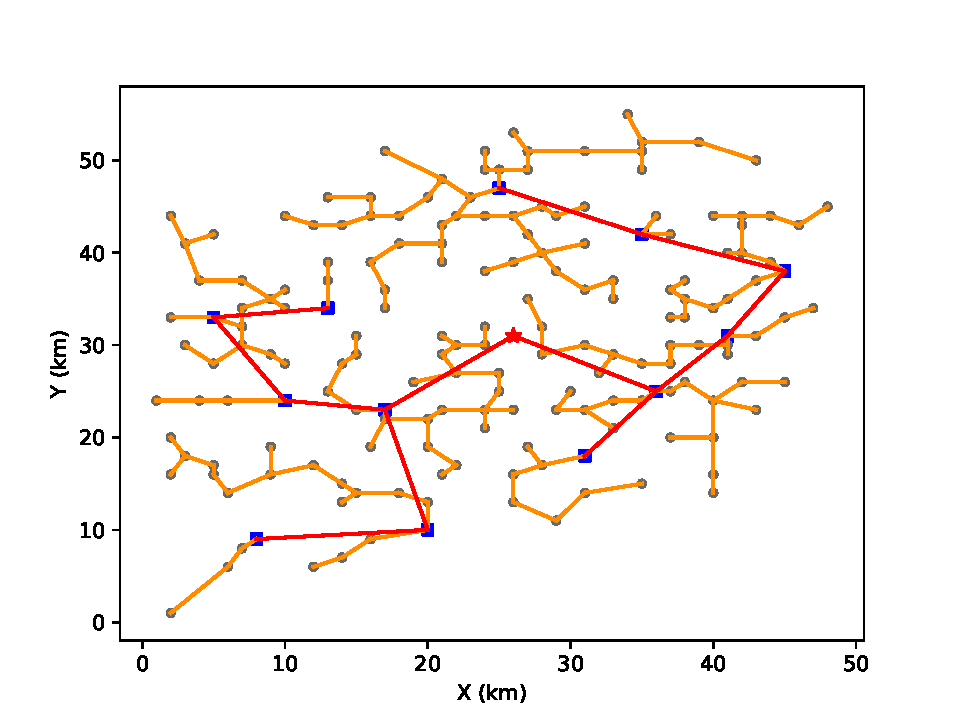
\includegraphics[width=.9\textwidth]{figure/pipeline.pdf}
    \caption{问题1结果}
    \label{fig:solution1}
  \end{figure}

我们还求得从各一级供水站输出的二级供水站个数以及的输出线路的总长度,如\cref{tab:001}所示;

\begin{table}[!h]
  \caption{每个一级供水站供给的二级供水站数量及其所属管道长度}\label{tab:001} \centering
  \begin{tabular}{ccccccccccccc}
      \toprule[1.5pt]
      水站id & 1 & 2 & 3 & 4 & 5 & 6 & 7 & 8 & 9 & 10 & 11 & 12\\
      \midrule[1pt]
      子站个数&16 & 3 & 3 & 2 & 24 & 17 & 46 & 7 & 2 & 16 & 15 & 17 \\
      线路总长&38.95 & 10.05 & 9.0 & 5.0 & 53.68 & 42.8 & 112.40 & 21.97 & 4.23 & 39.94 & 33.09 &32.25  \\
      \bottomrule[1.5pt]
  \end{tabular}
\end{table}

  经过加总可知:最优方案建设需要的最少一级管道总里程为120.94km,最少二级管道总里程为403.40km.


\section{问题三的模型建立与求解}
\subsection{问题三的描述与分析}
  在不升级任何二级供水站时,所有一级供水站面临的连接和负载情况,已在问题1中得出,如\cref{tab:001}所示:

    从中我们可以发现在该供水系统中,二级供水站与一级供水站的分布位置极不匹配,在第7号一级供水站周围的二级供水站过多,已经给一级供水站增加了许多负担,5、6号一级供水站铺设出的二级管道也超出了范围限制。
    我们接下来会对5、6、7号一级供水站周围的二级供水站进行细分或重新分配,希望保持升级数量较少的同时,满足功率限制。

\subsection{管道分支嫁接模型的建立}
  \subsubsection{最优子结构定理}
    \begin{theorem}
      最优子结构定理:如果一个问题的最优解中包含了子问题的最优解,则该问题具有最优子结构。
      \label{thm:best_sub}
    \end{theorem}
    
    证明如下:假设我们已经得到了一个最小生成树$T$,$(u,v)$是这棵树中的任意一条边:
    
    当把连接$u$,$v$的边去掉后(这条边是连接两棵树的最小边),得到两颗子树。
    
    
    $T_{1}$是图$G_{1}=(V_{1},E_{1})$的最小生成树,$G_{1}$是由$T_{1}$的顶点导出的图$G$的子图,$E_{1}={(x,y)\in E,x,y\in V_{1}}$同理可得$T_{2}$是$G_{2}=(V_{2},E_{2})$的最小生成树,$G_{2}$是由$T_{2}$的顶点导出的$G$的子图,
    $E_{2}={(x,y)\in E,x,y\in V_{1}}$
    结论证明:使用剪贴法,$w(T)$表示$T$树的权值和。
    权值关系满足:$$w(T)=w(u,v)+w(T_{1})+w(T_{2})$$
    假设有一棵树$T_{1}'$比$T_{1}$更适合图$G_{1}$,那么就存在$T'={(U,V)}\bigcup T_{1}'\bigcup T_{2}'$,那么$T'$就比$T$更适合图$G$,这与$T$是最优解相矛盾,\cref{thm:best_sub}得证。
    

    为了尽可能减少供水站的升级数,我们首先想到的是将超载供水站的连接负载重新分配,每个一级供水站的管道铺设情况已经如上图所示。

    在共$N$个一级供水站中,按照方案一中的管道建造计划,我们将每个管道子系统看做一棵树苗,对其枝条总长度,即二级管道总里程$TL_{i}(i=1,2...N)$进行由小到大的排序,若$TL_{i}>TL_{P},TL_{P}=40km$,则该树苗为被嫁接树苗,即需要减少管道总里程,其余树苗为嫁接树苗,需要平衡负载即增加管道长度。
    对嫁接树苗进行由小到大的重新排序,编号为$a_{1}$,$a_{2}$,....$a_{h}$,$h$为需要嫁接的树苗总数,其相应节点(二级供水站)编号$b_{i1}$,$b_{i2}$,....$b_{iq_{i}}$, $q_{i}$为相应树苗上的节点总数。
    根据两点间距离公式和最优子结构定理,我们在某一嫁接树苗上找到其与被嫁接树苗距离最近的节点,即使某一嫁接树苗上的节点与被嫁接树苗上的节点距离最近的一条线,根据最优子结构定理,嫁接部分可以沿着原线路继续延伸或者寻找新的被嫁接树苗上的节点。
  
    \begin{itemize}
    \item 新树苗需满足功率限制:
    $$TL_{i}'<=TL_{P}$$
    $TL_{i}'$为新树苗的枝条总长度,即新管道分支系统的总里程。
    \item 最佳的新树苗需满足枝条长度达到最长,即不会有其他任何可行的其他连接方式,使得该树苗的长度进一步增加而满足功率限制。
    
    \end{itemize}

    如果所有嫁接树苗都已达到最佳长度,仍有至少一个树苗不满足功率限制,则此时,应对系统进行升级。
 
\subsection{问题三模型的求解}
  各水站负载线路总长度,即所有一级供水站和二级管道输出II级水管线路总长度示意图如\cref{fig:pipline_length}。
  \begin{figure}[!h]
    \centering
    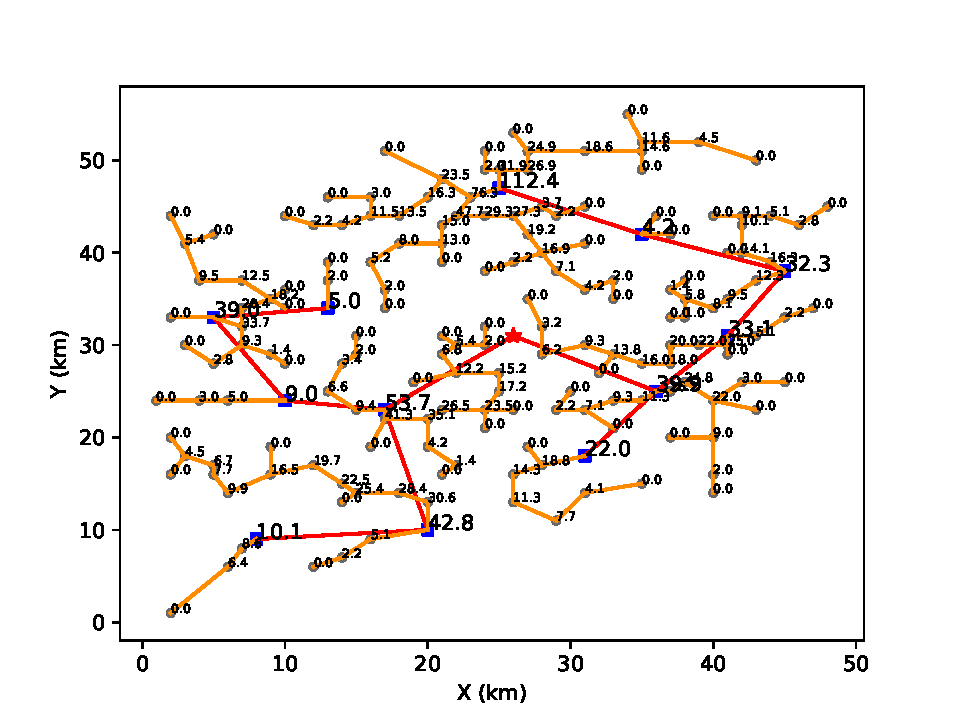
\includegraphics[width=.8\textwidth]{figure/pipline_length.pdf}
    \caption{各水站负载线路总长度}
    \label{fig:pipline_length}
  \end{figure}
  嫁接开始前先求出所有超载的一级水站和其所有子水站列表$overloadStation[]$,此列表长度为超载的一级水站的个数,每个元素为一个集合,包含一级水站和其所有子水站。

  开始第一步嫁接,先求出所有负载未达最大负载$MAX_LOAD$的一级水站和其所有子水站$availableStation[]$,此列表长度为有余闲的一级水站的个数,每个元素为一个集合,包含一级水站和其所有子水站。按照其余闲的负载$availableLoad[]$降序排列。
  
  从余闲的负载最大的一级水站$availableIStation[i]$开始遍历$availableIStation[]$在\cref{fig:pipline_graft_connection_0}。$availableIStation[i]$如图\cref{fig:pipline_graft_connection_0}中绿色圈所示。
  
  下面筛选可能与$availableIStation[i]$嫁接的所有超载树中的水站。
  筛选出二级水站的集合为:
  $$overloadStation={P[i] |P[i].load < availableIStation[i].availableLoad }$$
  即$P[i]$的负载小于可嫁接树的剩余负载。如图\cref{fig:pipline_graft_connection_0}中红色圈所示。

  选取权值最小的边$<u, v>$,其中$u \in availableIStation[i]$,而$v \in overloadStation$
  作为嫁接的连接点。如图\cref{fig:pipline_graft_connection_0}中绿色虚线所示。

  \begin{figure}[!h]
    \centering
    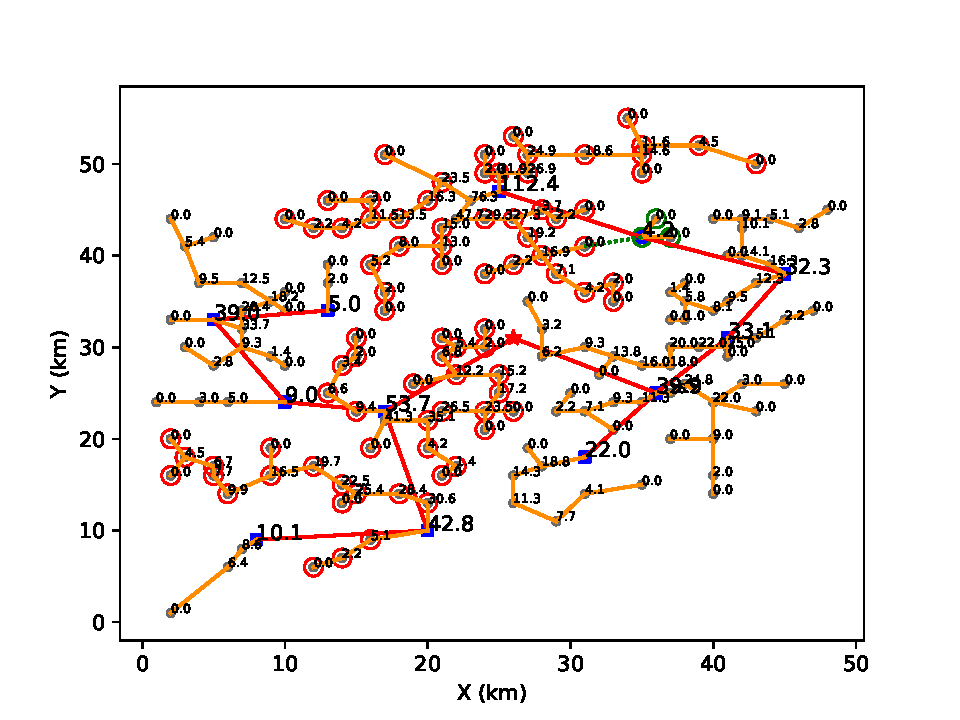
\includegraphics[width=.95\textwidth]{figure/pipline_graft_connection_0.pdf}
    \caption{第1次嫁接的候选水站和执行嫁接连接的两个水站}
    \label{fig:pipline_graft_connection_0}
  \end{figure}
  从$v$开始逐渐追溯其父节点(输入水源的供水站),搜索嫁接部分和超载树之间的切割边$cutEdge=<u_c, v_c>$。使$cutEdge$满足:
  $$u_c.load + distanceMat[u, v]>availableIStation[i].availableLoad$$
  $$v_c.load + distanceMat[u, v]<=availableIStation[i].availableLoad$$
  $cutEdge$中,$u_c$为父节点,$v_c$为子节点,即水流从$u_c$流向$v_c$。$cutEdge$如图\cref{fig:pipline_graft_cut_0}中用无橙色底色的绿色虚线所示。
  \begin{figure}[!h]
    \centering
    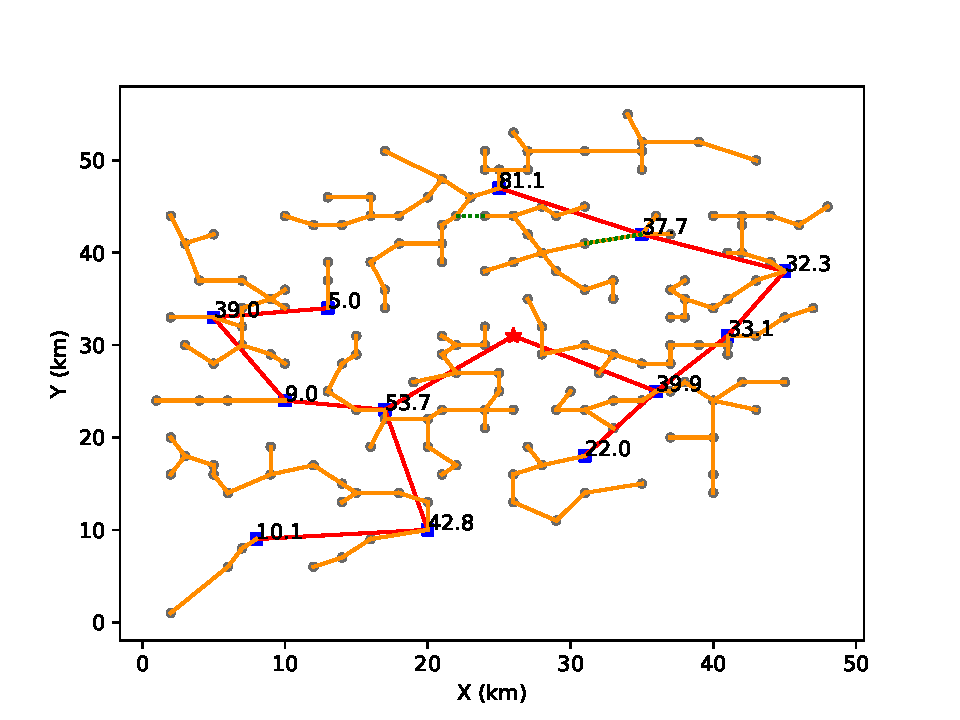
\includegraphics[width=.95\textwidth]{figure/pipline_graft_cut_0.pdf}
    \caption{第1次嫁接断开的边以及嫁接后个一级水站的负载}
    \label{fig:pipline_graft_cut_0}
  \end{figure}

  到此为止视为完成一次嫁接,更新一次所有水站的连接状态树后:
  \begin{itemize}
    \item 更新最小生成树树的连接结构参数。
    \item 更新$overloadStation[]$和$availableIStation[i]$
  \end{itemize}
  遍历进行第二次嫁接,结果如\cref{fig:pipline_graft_connection_1},\cref{fig:pipline_graft_cut_1}。

  \begin{figure}[!h]
    \centering
    \begin{minipage}[c]{0.45\textwidth}
        \centering
        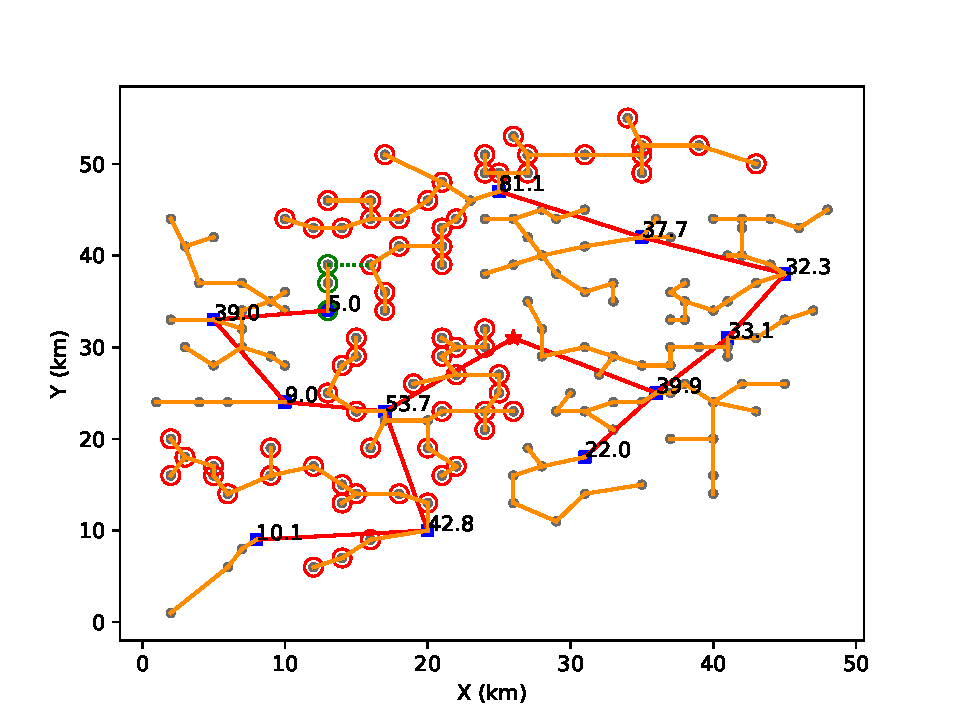
\includegraphics[width=0.99\textwidth]{figure/pipline_graft_connection_1.pdf}
        \subcaption{第2次嫁接的候选水站和$<u, v>$}
        \label{fig:pipline_graft_connection_1}
    \end{minipage}
    \begin{minipage}[c]{0.45\textwidth}
        \centering
        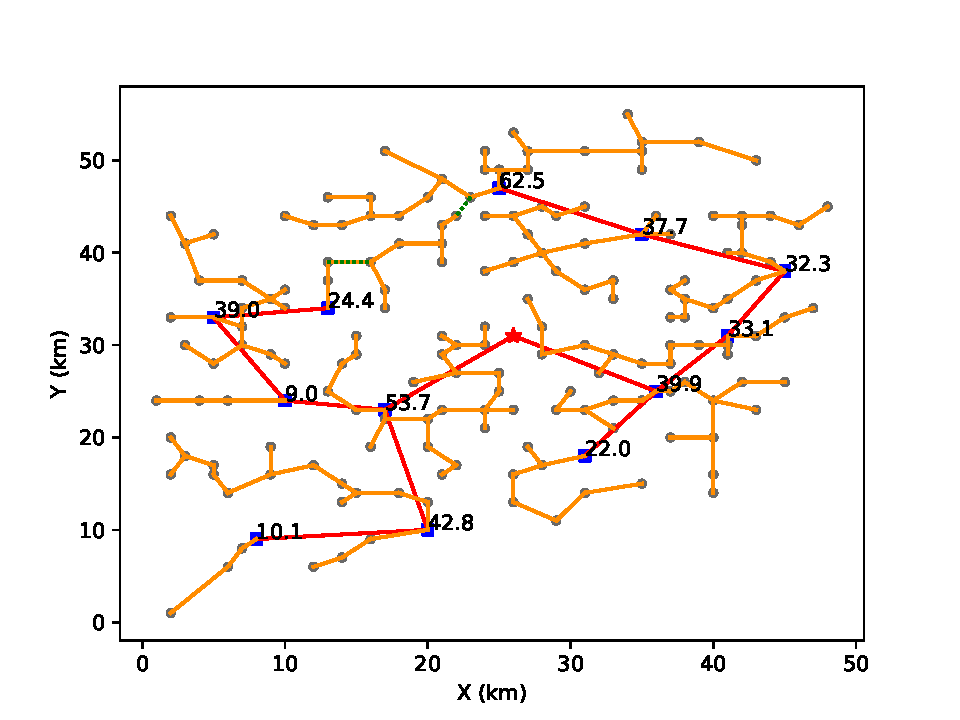
\includegraphics[width=0.99\textwidth]{figure/pipline_graft_cut_1.pdf}
        \subcaption{第2次嫁接断开的边}
        \label{fig:pipline_graft_cut_1}
    \end{minipage}
  \end{figure}
  第3到8次嫁接。

  \begin{figure}[!h]
    \centering
    \begin{minipage}[c]{0.45\textwidth}
        \centering
        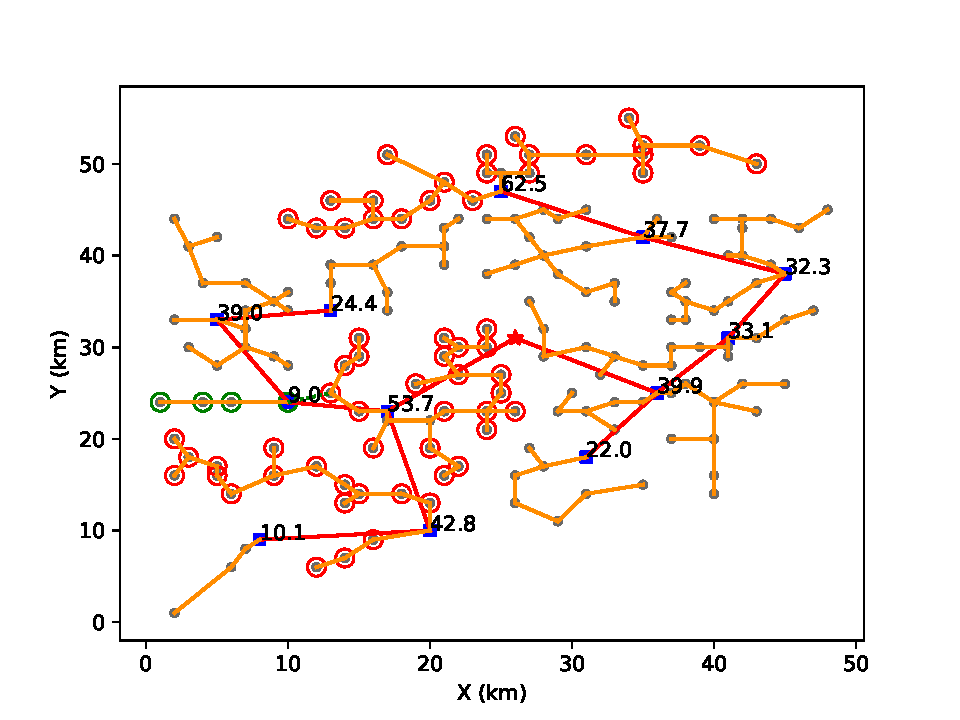
\includegraphics[width=0.99\textwidth]{figure/pipline_graft_connection_2.pdf}
        \subcaption{第3次嫁接的候选水站和$<u, v>$}
        \label{fig:pipline_graft_connection_2}
    \end{minipage}
    \begin{minipage}[c]{0.45\textwidth}
        \centering
        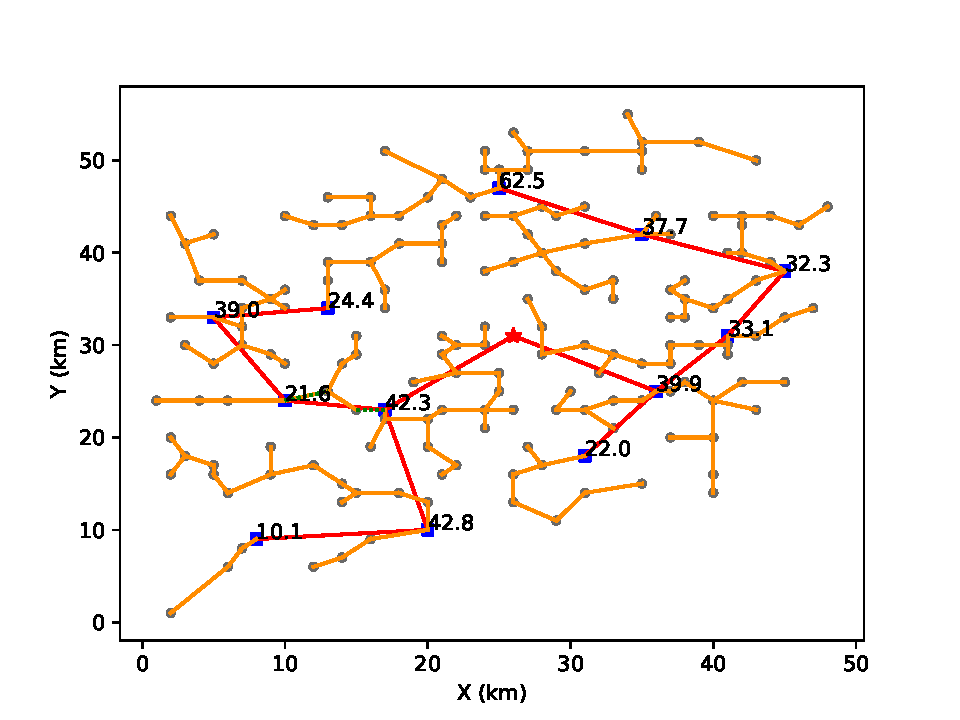
\includegraphics[width=0.99\textwidth]{figure/pipline_graft_cut_2.pdf}
        \subcaption{第3次嫁接断开的边}
        \label{fig:pipline_graft_cut_2}
    \end{minipage}
  \end{figure}
  
  \begin{figure}[!h]
    \centering
    \begin{minipage}[c]{0.45\textwidth}
        \centering
        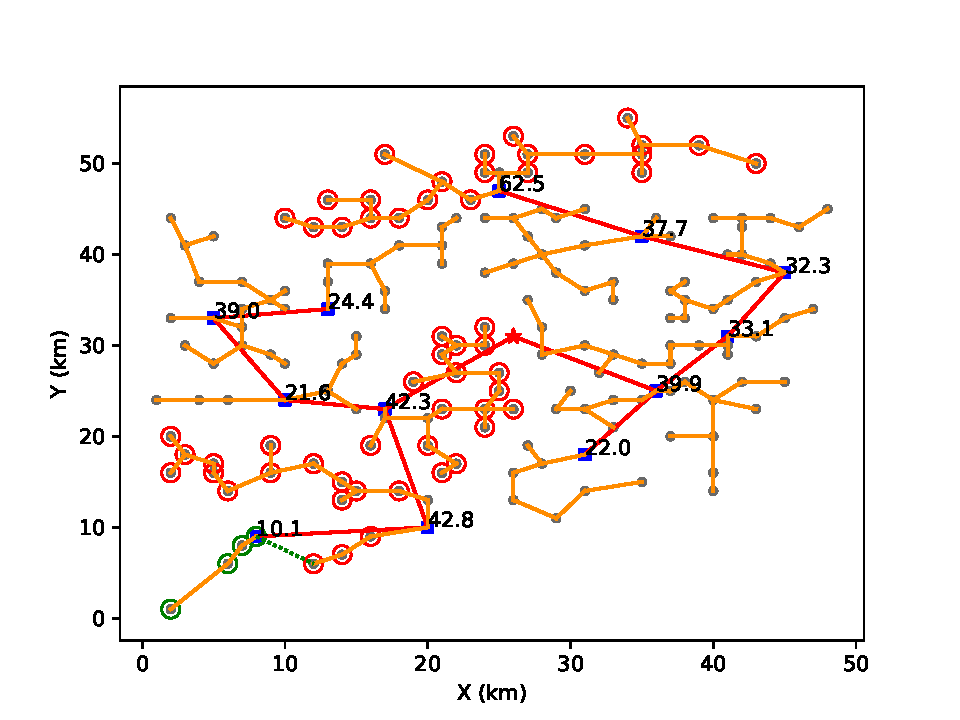
\includegraphics[width=0.99\textwidth]{figure/pipline_graft_connection_3.pdf}
        \subcaption{第4次嫁接的候选水站和$<u, v>$}
        \label{fig:pipline_graft_connection_3}
    \end{minipage}
    \begin{minipage}[c]{0.45\textwidth}
        \centering
        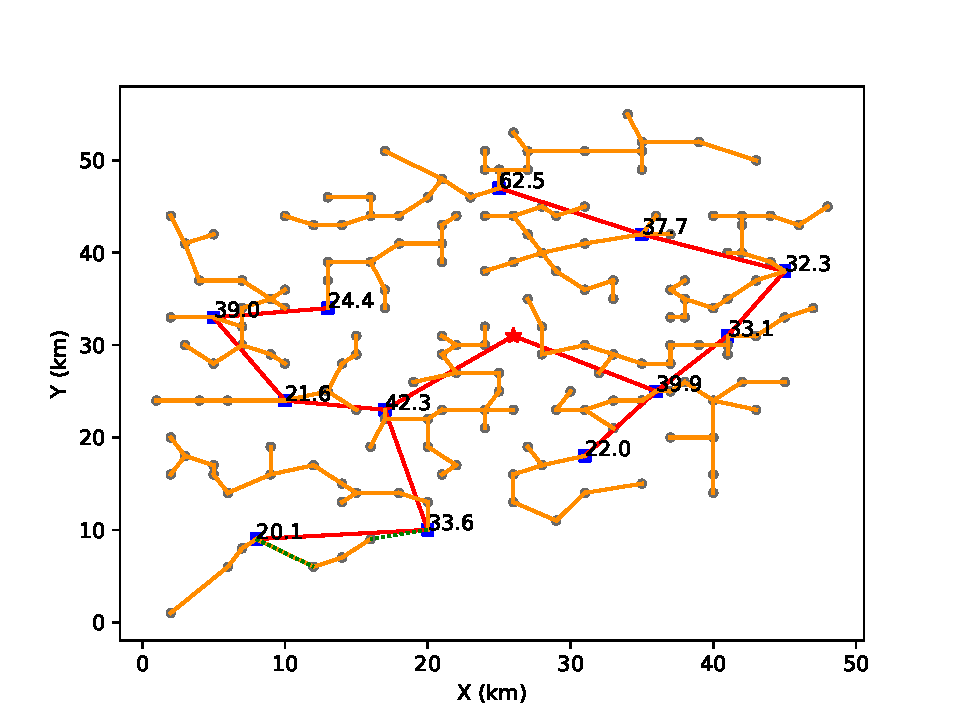
\includegraphics[width=0.99\textwidth]{figure/pipline_graft_cut_3.pdf}
        \subcaption{第4次嫁接断开的边}
        \label{fig:pipline_graft_cut_3}
    \end{minipage}
  \end{figure}
  
  \begin{figure}[!h]
    \centering
    \begin{minipage}[c]{0.45\textwidth}
        \centering
        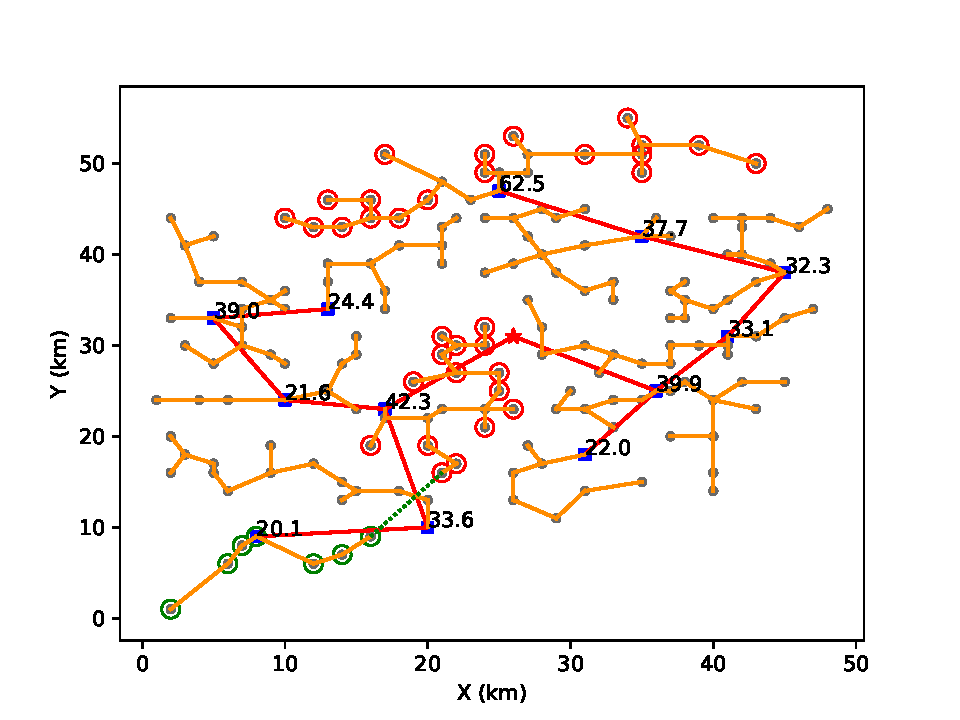
\includegraphics[width=0.99\textwidth]{figure/pipline_graft_connection_4.pdf}
        \subcaption{第5次嫁接的候选水站和$<u, v>$}
        \label{fig:pipline_graft_connection_4}
    \end{minipage}
    \begin{minipage}[c]{0.45\textwidth}
        \centering
        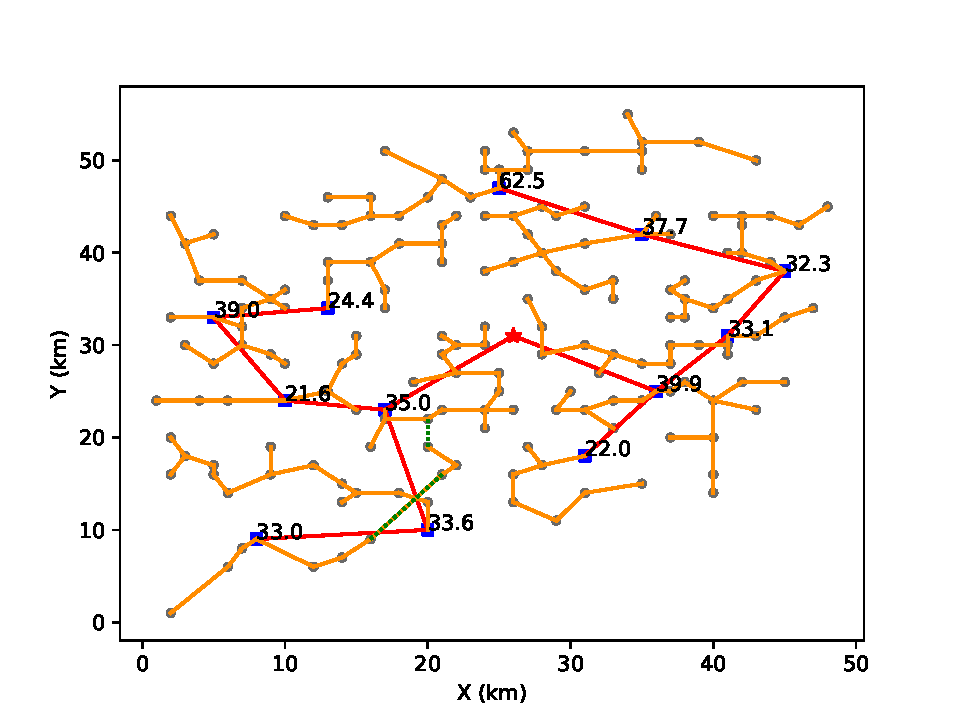
\includegraphics[width=0.99\textwidth]{figure/pipline_graft_cut_4.pdf}
        \subcaption{第5次嫁接断开的边}
        \label{fig:pipline_graft_cut_4}
    \end{minipage}
  \end{figure}
  
  \begin{figure}[!h]
    \centering
    \begin{minipage}[c]{0.45\textwidth}
        \centering
        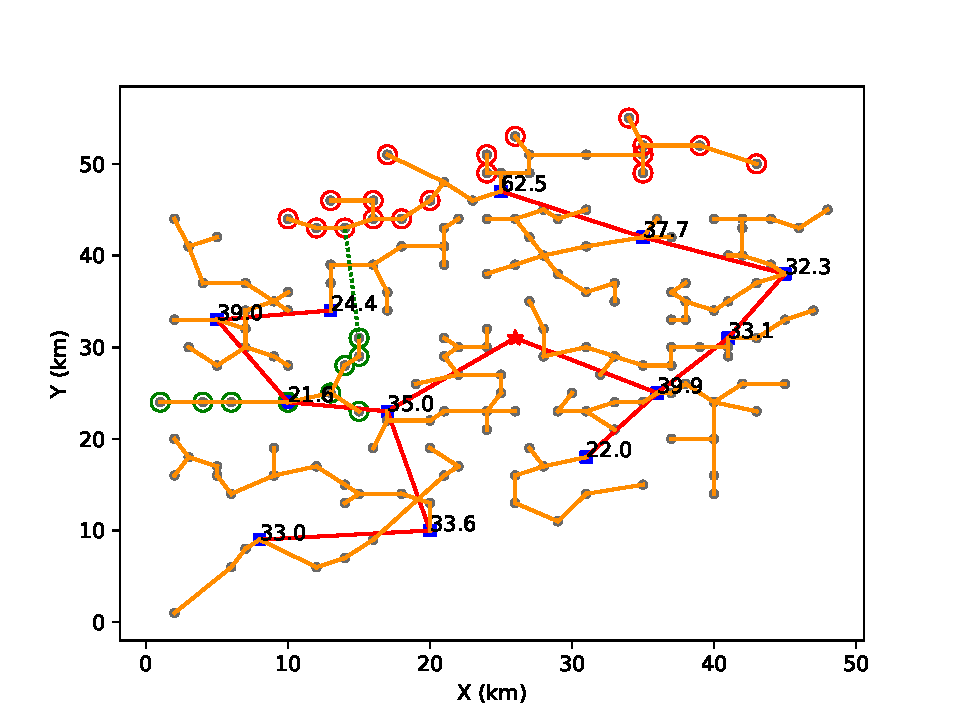
\includegraphics[width=0.99\textwidth]{figure/pipline_graft_connection_5.pdf}
        \subcaption{第6次嫁接的候选水站和$<u, v>$}
        \label{fig:pipline_graft_connection_5}
    \end{minipage}
    \begin{minipage}[c]{0.45\textwidth}
        \centering
        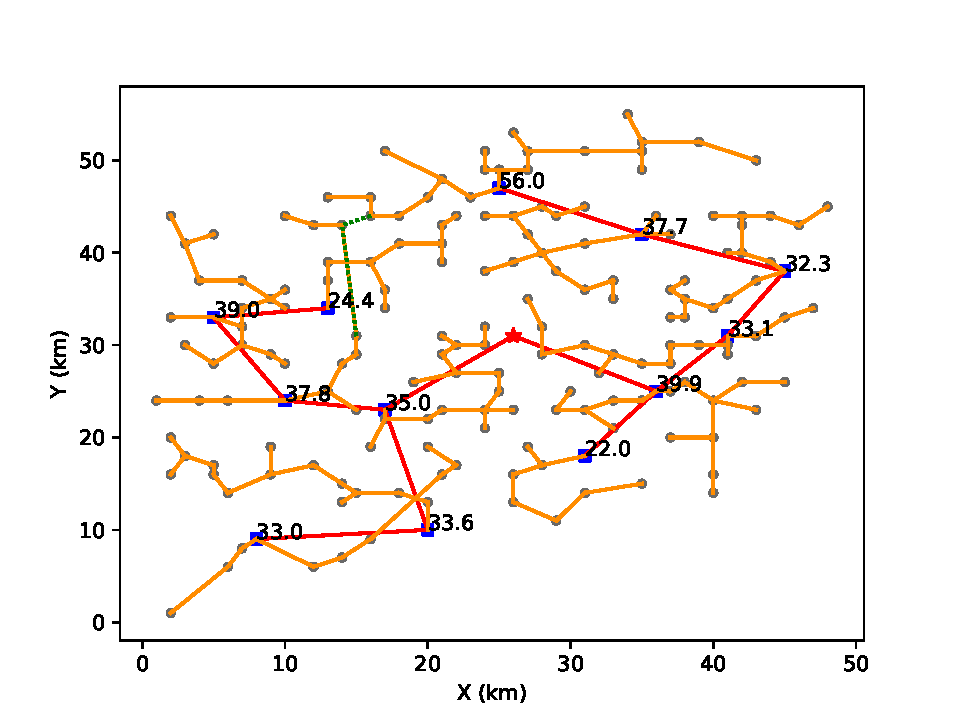
\includegraphics[width=0.99\textwidth]{figure/pipline_graft_cut_5.pdf}
        \subcaption{第6次嫁接断开的边}
        \label{fig:pipline_graft_cut_5}
    \end{minipage}
  \end{figure}
  
  \begin{figure}[!h]
    \centering
    \begin{minipage}[c]{0.45\textwidth}
        \centering
        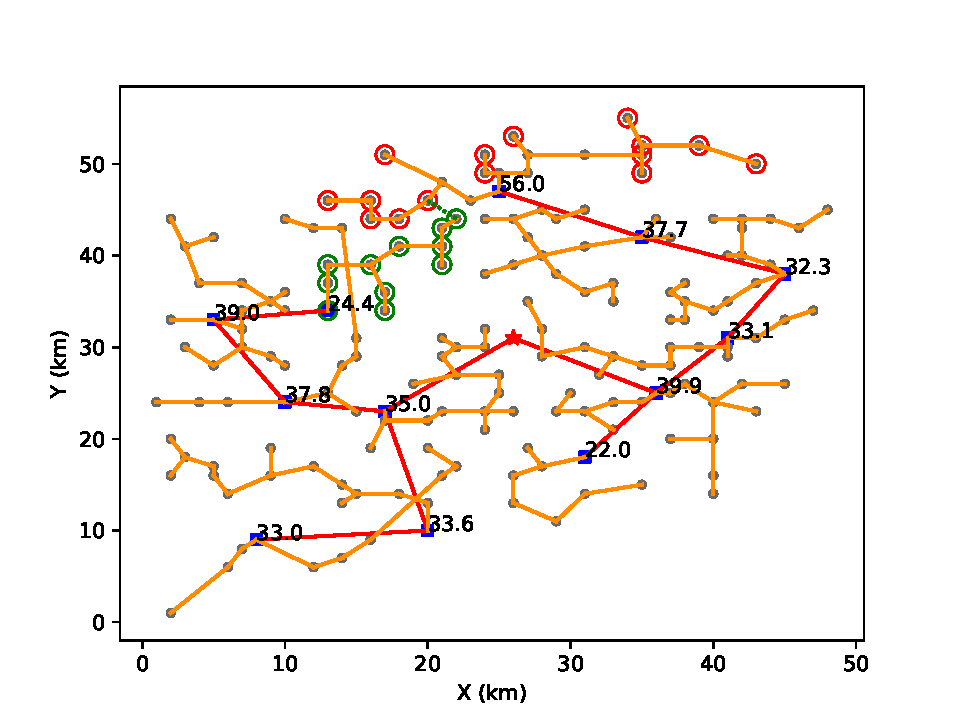
\includegraphics[width=0.99\textwidth]{figure/pipline_graft_connection_6.pdf}
        \subcaption{第7次嫁接的候选水站和$<u, v>$}
        \label{fig:pipline_graft_connection_6}
    \end{minipage}
    \begin{minipage}[c]{0.45\textwidth}
        \centering
        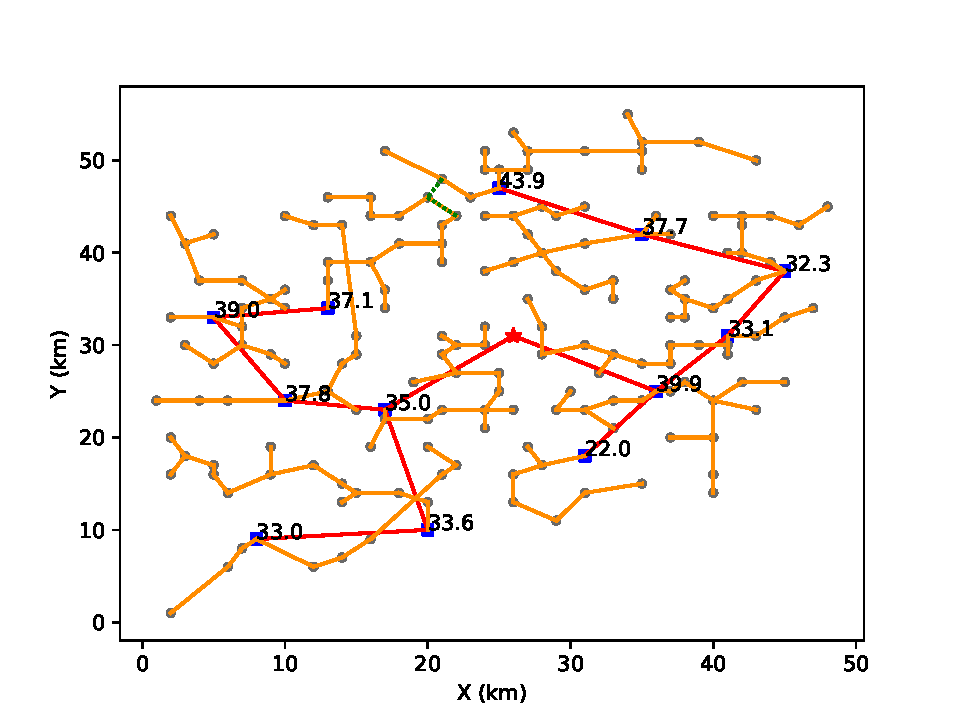
\includegraphics[width=0.99\textwidth]{figure/pipline_graft_cut_6.pdf}
        \subcaption{第7次嫁接断开的边}
        \label{fig:pipline_graft_cut_6}
    \end{minipage}
  \end{figure}
  
  \begin{figure}[!h]
    \centering
    \begin{minipage}[c]{0.45\textwidth}
        \centering
        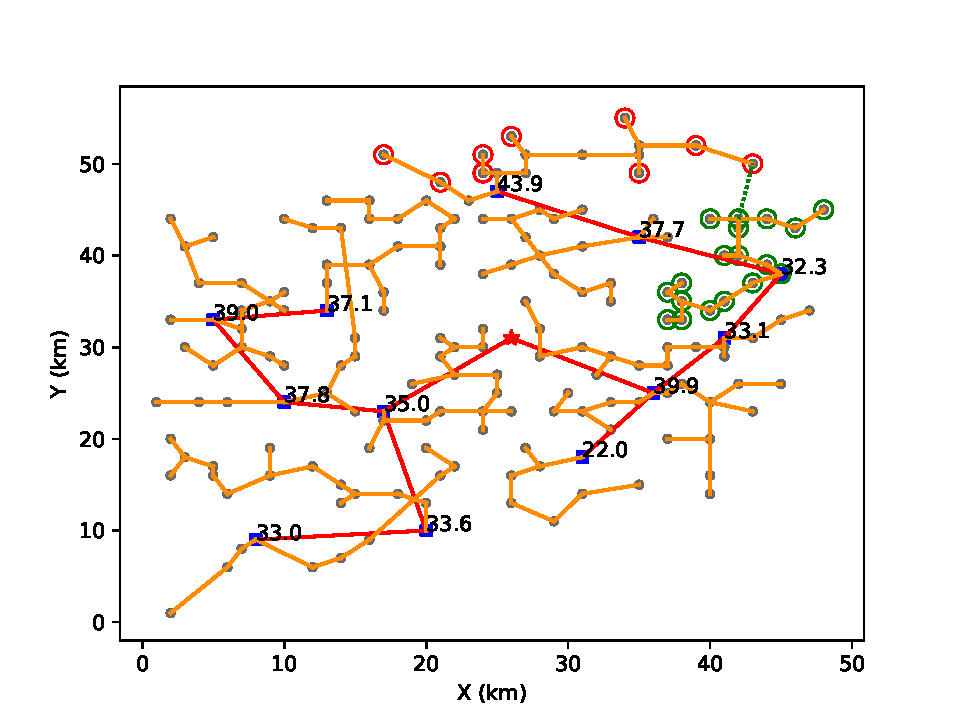
\includegraphics[width=0.99\textwidth]{figure/pipline_graft_connection_7.pdf}
        \subcaption{第8次嫁接的候选水站和$<u, v>$}
        \label{fig:pipline_graft_connection_7}
    \end{minipage}
    \begin{minipage}[c]{0.45\textwidth}
        \centering
        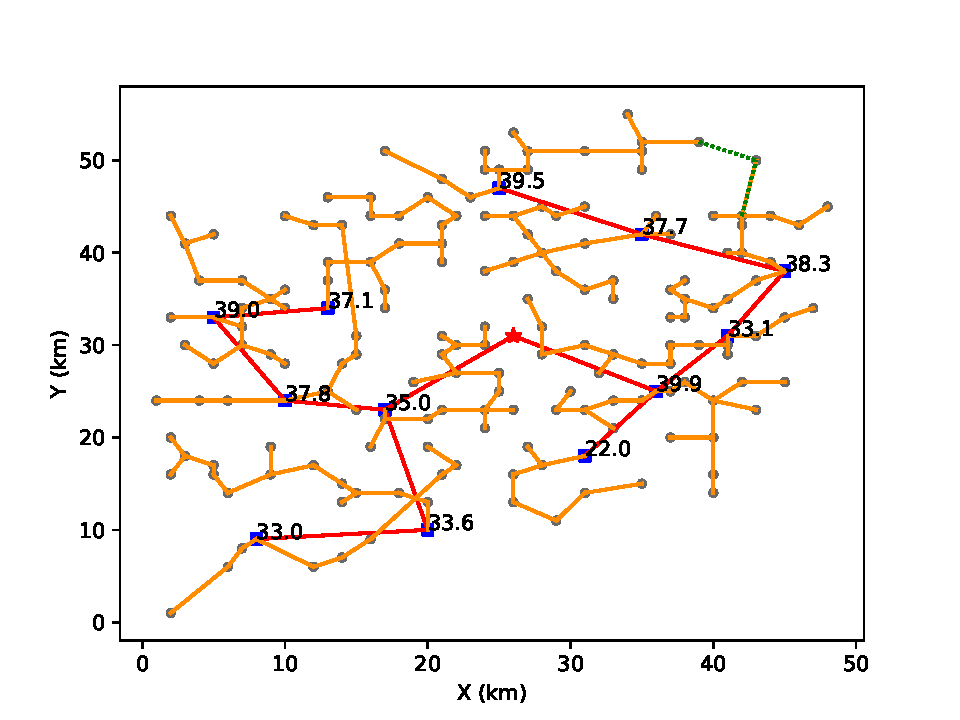
\includegraphics[width=0.99\textwidth]{figure/pipline_graft_cut_7.pdf}
        \subcaption{第8次嫁接断开的边}
        \label{fig:pipline_graft_cut_7}
    \end{minipage}
  \end{figure}
最终
嫁接后II级水管总长:425.94km。如\cref{fig:pipline_graft_cut_9}
\begin{figure}[!h]
  \centering
  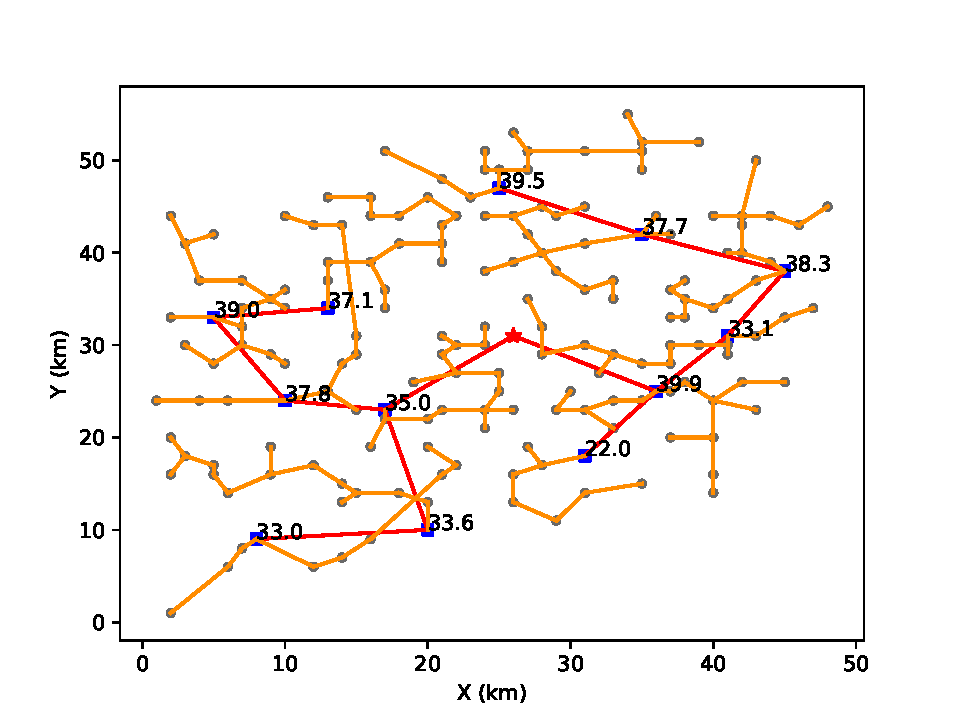
\includegraphics[width=.9\textwidth]{figure/pipline_graft_cut_9.pdf}
  \caption{问题3结果}
  \label{fig:pipline_graft_cut_9}
\end{figure}

\newpage

\section{模型总结与评估}
\subsection{优点}
\begin{itemize}
\item 在构建最优管道系统时,Prim算法可以寻找在当前情况下的最优解,并将新的站点纳入系统,在应对稠密多个连接点系统时具有优势。
\item 嫁接法兼顾了管线长度最小和一级水站的负载均衡,充分利用水站的空余负载,达到尽量减少升级水站数目的目的。
\end{itemize}
\subsection{缺点}
\begin{itemize}
\item Prim算法在进行边的选择时,会遍历所有边线,这样会导致算法具有较高时间复杂度。
\item

\end{itemize}
%参考文献
\section{参考文献}
\newpage
%附录
\begin{appendices}
  \section{Python源代码}
  \begin{lstlisting}[language=python]
  \end{lstlisting}

\end{appendices}

\end{document} 
